\section{Execution}
\subsection{Upload Code to Arduino}
\begin{enumerate}
    \item Connect Arduino to computer via USB
    \item Upload the following code to the Arduino using PlatformIO.
	%{\em Platformio}.
\fbox{\parbox{\linewidth}{\url{https://github.com/gadepall/clock/blob/main/codes/code.cpp}
}}
\item Open PlatformIO, select New Project and then fill in the details (name, board \& framework).
\item Then replace contents in src/main.cpp with the above code, now run \& upload that code to Arduino Uno.
\end{enumerate}

\subsection{Hardware Build}
\begin{enumerate}
    \item Connect the seven-segment displays to the breadboard
    \item Connect all segment outputs together (through resistors)
    \item Make connections to the IC7447 according to Table 3.0
    \item Connect the IC7447 and the buttons to the Arduino according to Table 2.0
    \item Add appropriate current-limiting resistors for LEDs and pull-down resistors for buttons
\end{enumerate}

\begin{figure}[ht]
\centering
\includegraphics[width=0.5\textwidth]{figs/clock.jpg}
\caption{Final Arduino-based Clock Implementation}
\end{figure}

\begin{figure}[ht]
\centering
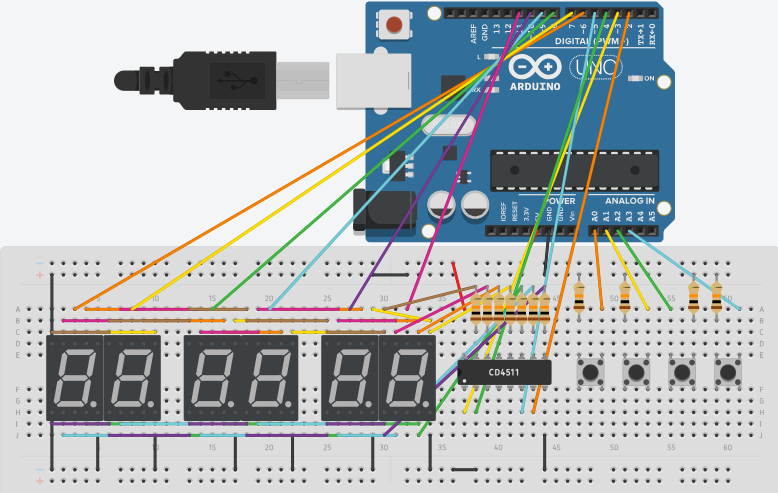
\includegraphics[width=0.45\textwidth]{figs/Clock_Tinkercad.png}
\caption{Tinkercad Simulation of the Digital Clock}
\end{figure}
